\section{Periodic layers}\label{sec:layers}

Our goal is to replace the closed walks of the base graph by ordered layers without changing any edge. Their actual windows will later provide the occurrence records and same-text joins used to spend the second $W$ budget.

\subsection{Lifting closed walks to windows}

Decompose the balanced base graph into nonempty closed walks. Every such walk has the same positive number of up and down steps: the word length changes by $+1$ or $-1$ at each step and returns to its starting value. Read the letters appended on the up steps cyclically, and repeat this circular word in both directions to obtain a periodic text.

On the infinite repetition of the walk, represent a vertex by a window $[x,e)$ of this text. An up step increases $e$ by one; a down step increases $x$ by one. The window spells the vertex word. To verify this last assertion, follow the repeated walk sufficiently far back: its down steps eventually remove every letter previously present, so each current letter must have entered at one of the indicated up steps. A closed walk with $P$ up steps advances both coordinates by $P$.

An occurrence interval of a nonempty word $s$ is \emph{recorded} on the walk if some visited window contains it. Count occurrences modulo the walk's turn length $P$, so each starting-position residue contributes at most once. Here the modulus is $P$, even if the text has a smaller least period.

\begin{lemma}\label{lem:recorded}
The total number of recorded occurrences of $s$ on all the closed walks is $m(s)$.
\end{lemma}

\begin{proof}
At the unique up step reaching the right endpoint of a given occurrence, the current window contains the occurrence if and only if it is recorded. Indeed, subsequent left endpoints only increase, so a later containing window implies containment at that step as well. The up step generates a word ending in $s$. Summing its multiplicity over all such words gives
\[
\sum_{r\in V:\ r\text{ ends in }s}u(r)=m(s)
\]
by telescoping over left extensions in \eqref{eq:base-multiplicities}. The argument is on the infinite lift and therefore also applies when $\len s$ exceeds a turn length.
\end{proof}

\subsection{Sorting primitive passages}

Group the walks by their periodic texts up to integer translation, and align the texts within each group. Group membership is up to translation, while a later record compares a specified coordinate alignment of two layers; that alignment can differ even within one group. Write $p$ for the least positive period of a group. Every original turn length is a multiple of $p$: the shifts preserving a two-sided text form a subgroup of $\ZZ$, generated by its least positive member.

\begin{lemma}[Ordered layers]\label{lem:layers}
The walks of a group can be rearranged, without changing the multiset of their graph edges, into one-turn layers of period $p$. Each layer has an integer function $z:\ZZ\to\ZZ$ such that
\begin{equation}\label{eq:layer-properties}
z(x-1)\le z(x),\qquad z(x-1)\ge x,
\qquad z(x+p)=z(x)+p.
\end{equation}
At start coordinate $x$, its windows are exactly
\begin{equation}\label{eq:layer-vertical}
[x,e),\qquad z(x-1)\le e\le z(x);
\end{equation}
it then takes a down step to start $x+1$. The functions of the layers in a group are pointwise ordered. Each layer has up cost $p$, and the sum of these costs over all groups is $W$.
\end{lemma}

\begin{proof}
For original walk $j$, let $P_j=d_jp$ be its turn length and let $Z_j(x)$ be its exit end at start $x$ on the infinite lift. Thus $Z_j(x+P_j)=Z_j(x)+P_j$. At each integer start $x$, collect the normalized exit ends
\[
\mathcal E_x=
\bigl\{Z_j(x+rp)-rp:\ j,\ 0\le r<d_j\bigr\},
\]
with multiplicity. These are the passages through the same start residue, translated to start $x$. Translation by $rp$ preserves their word labels. Sort $\mathcal E_x$ increasingly and call its order statistics $z_1(x),\ldots,z_h(x)$, where $h=\sum_j d_j$.

The corresponding entering ends at $x$ form $\mathcal E_{x-1}$. Each original exit is at least its paired entry, so the increasing order statistics also satisfy $z_i(x-1)\le z_i(x)$. Every entry is at least $x$. Moreover, increasing $x$ by $p$ permutes the passages from each original walk and adds $p$ to their ends. Thus $\mathcal E_{x+p}=\mathcal E_x+p$, proving all of \eqref{eq:layer-properties}.

The multiset of down steps is fixed by the exit-end multisets. At a fixed $x$, the number of copies of a vertical unit edge with lower end $e$ is the number of entries at or below $e$ minus the number of exits at or below $e$. Thus the up-edge multiset is unchanged as well. The sorted passages therefore use exactly the original graph edges, with multiplicity, and in particular only actual base vertices. Each layer advances both coordinates by $p$ in one turn and has $p$ up steps. Their total up cost remains $W$.
\end{proof}

We henceforth use this fixed layer decomposition. A layer of period $p$ receives an additional \emph{budget} $p$. Budgets belong to layers even when several layers happen to share graph vertices.

For a layer $i$, write
\begin{equation}\label{eq:first-last}
f_i(x)=z_i(x-1),\qquad l_i(x)=z_i(x)
\end{equation}
for its first and last ends at start $x$. A higher layer has both functions at least those of a lower layer. When a collection of layers is under discussion, the subscripts $H$ and $L$ denote its highest and lowest layers; a scalar such as $H=f_H(t)$ denotes an end coordinate. \Cref{fig:layers} shows the first and last ends in start--end coordinates. Every actual window on a layer is a graph vertex in $V$; two windows that spell the same word are the same graph vertex, even when they have different coordinates.

\begin{figure}[htbp]
\centering
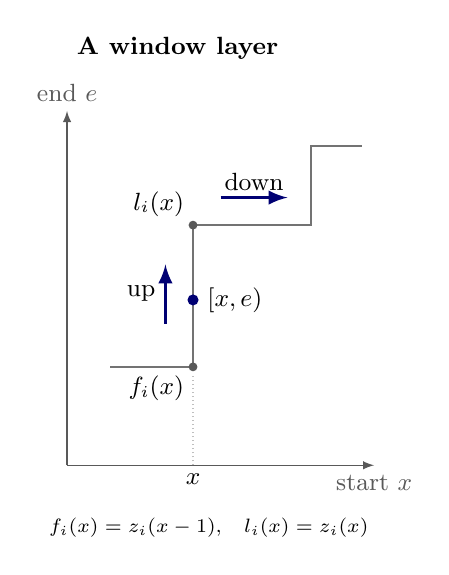
\begin{tikzpicture}[font=\small,>=latex,
  layer/.style={line width=.65pt,draw=black!55},
  connection/.style={line width=1.35pt,draw=blue!45!black},
  guide/.style={draw=black!25,densely dotted,line width=.45pt}]

  \begin{scope}[shift={(0,.75)}]
    \node[anchor=west,font=\small\bfseries] at (0,5.3) {A window layer};
    \draw[->,black!65] (0,0) -- (3.9,0) node[below] {start $x$};
    \draw[->,black!65] (0,0) -- (0,4.5) node[above] {end $e$};
    \draw[layer] (.55,1.25) -- (1.6,1.25) -- (1.6,3.05)
      -- (3.1,3.05) -- (3.1,4.05) -- (3.75,4.05);
    \fill[black!65] (1.6,1.25) circle (1.6pt);
    \fill[black!65] (1.6,3.05) circle (1.6pt);
    \node[anchor=north east,inner sep=3pt] at (1.6,1.25) {$f_i(x)$};
    \node[anchor=south east,inner sep=3pt] at (1.6,3.05) {$l_i(x)$};
    \draw[connection,->] (1.25,1.8) -- (1.25,2.55)
      node[midway,left,inner sep=3pt] {up};
    \draw[connection,->] (1.95,3.4) -- (2.8,3.4)
      node[midway,above,inner sep=2pt] {down};
    \fill[blue!45!black] (1.6,2.1) circle (2pt);
    \node[anchor=west,inner sep=5pt] at (1.6,2.1) {$[x,e)$};
    \draw[guide] (1.6,0) -- (1.6,1.17);
    \node[below,inner sep=3pt] at (1.6,0) {$x$};
    \node[anchor=north,align=center,font=\scriptsize] at (1.8,-.55)
      {$f_i(x)=z_i(x-1)$,\quad $l_i(x)=z_i(x)$};
  \end{scope}

\end{tikzpicture}

\caption{A layer in start--end coordinates. An up step appends a letter and increases the end; a down step deletes the first letter and increases the start. At start $x$, the layer visits every window $[x,e)$ between its first end $f_i(x)$ and its last end $l_i(x)$.}
\label{fig:layers}
\end{figure}

\subsection{Unblocked occurrences on layers}

Align a recorded occurrence of $s$ on a layer with a template $A$ containing $s$ at position zero. Call it blocked if the interval from the nearest left mismatch to the nearest right mismatch is itself recorded on that layer. Such a block automatically belongs to $V$, since it is a substring of a visited window.

\begin{lemma}[Matching window]\label{lem:matching-window}
Over all layers, the number of blocked occurrences of $s$ relative to $A$ is $B_A(s;m)$. Every unblocked occurrence is contained in an actual layer window that agrees with $A$ throughout.
\end{lemma}

\begin{proof}
Each recorded occurrence of a word $r$ counted in \eqref{eq:block-functional}, together with a counted placement of $s$ in it, gives a blocked occurrence. Conversely, the nearest mismatch pair uniquely determines $r$ and its placement. This correspondence commutes with translation by one layer turn, so it is a bijection also for the occurrences counted modulo that turn. \Cref{lem:recorded} gives the asserted count. Sorting layers did not change that lemma, since it preserved all base edges.

For the second assertion, write the selected occurrence as $[u,v)$. Its first containing window is reached by the up step with end $v$, so that window contains no right mismatch. If it has no left mismatch either, it suffices. Otherwise let $\ell<u$ be the nearest left mismatch. Follow the layer until a down step removes $\ell$; this happens while the windows still contain $[u,v)$, since their starts eventually reach $u$. No right mismatch can enter before that step: together with $\ell$ it would make the nearest-mismatch bracket a recorded interval, contrary to the occurrence being unblocked. The down step introduces no new letter. Immediately afterward no mismatch remains on either side, and the resulting actual window agrees throughout with $A$.
\end{proof}

In particular,
\begin{equation}\label{eq:unblocked-count}
m(s)-B_A(s;m)
\end{equation}
counts unblocked recorded occurrences. A layer whose entire text is the aligned template has no blocked occurrences relative to that template.

\subsection{Two periodicity facts}

Periodicity and extremal rotations also enter earlier superstring cycle-cover analyses~\cite{breslauer1997,mucha2013}. We prove the exact agreement and maximal-rotation statements needed here. Use the total order on $\Sigma$ induced by the encoded symbol labels. The lexicographic order of infinite forward words is determined by their first differing letter; equality means agreement at every nonnegative position. In a periodic group, a \emph{distinguished position} $t$ starts its lexicographically greatest forward rotation.

The agreement bound below uses only the weaker $p+q$ consequence of
Fine--Wilf periodicity~\cite{finewilf}; we retain its direct proof here.

\begin{lemma}[Agreement bounds]\label{lem:agreement}
Two distinct aligned periodic texts of periods $p,q$ agree on fewer than $p+q$ consecutive letters. If both have period $p$, they agree on fewer than $p$ consecutive letters.
\end{lemma}

\begin{proof}
Suppose that a period-$p$ text and a period-$q$ text agree on an interval of length $p+q$. For a full set of $q$ consecutive residues, both positions $i$ and $i+p$ lie in that interval. Equality with the first text therefore makes the second invariant under shift by $p$ at those residues, and $q$-periodicity extends this invariance everywhere. Both texts now have period $p$, and agreement for $p$ consecutive letters makes them equal. The same final observation proves the equal-period bound.
\end{proof}

\begin{lemma}[Maximal rotation]\label{lem:max-rotation}
Let $A$ have least period $p$, and let $t$ be distinguished. Let $D$ be a distinct aligned periodic text of period $q$, all of whose forward rotations are lexicographically at most the forward word of $A$ at $t$. Then $D$ and $A$ cannot agree on all $q$ positions starting at $t$.
\end{lemma}

\begin{proof}
Set $t=0$ by translating coordinates, and let $S$ be the forward word of $A$. It is at least its shift by $q$. If they are equal, $A$ has period $q$, and any period-$q$ text agreeing on the first $q$ letters is the identical aligned text.

Otherwise let $j\ge0$ be the first index at which $S(j)\ne S(j+q)$. Maximality gives $S(j)>S(j+q)$. Let $U$ repeat the first $q$ letters of $S$. The equalities $S(i)=S(i+q)$ for $i<j$ imply that $U$ and $S$ agree before index $j+q$. At that index,
\[
U(j+q)=U(j)=S(j)>S(j+q),
\]
so $U>S$. If $D$ agreed on the first $q$ letters, its forward word there would be $U$, contrary to the hypothesis on its rotations.
\end{proof}
